\usetikzlibrary{patterns, calc}


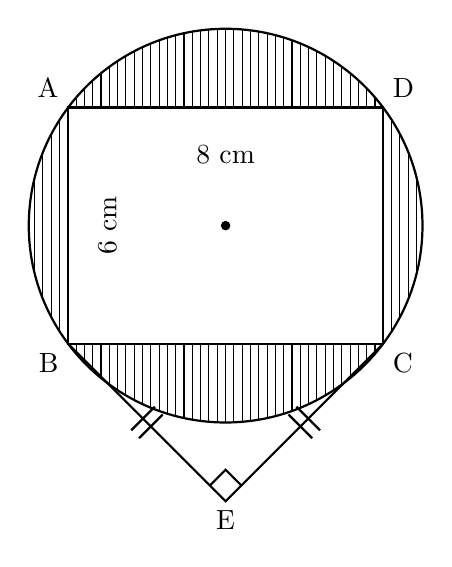
\begin{tikzpicture}[scale=1]

    % Define the center of the circle
    \coordinate (O) at (0,0);

    % Define the vertices of the rectangle inside the circle
    % The text says "8 cm" (top) and "6 cm" (left)
    % A 8x6 rectangle has a diagonal of 10, so the circumcircle radius is 5.
    % We scale this down by a factor of 0.5 to fit nicely.
    % Scaled width = 4, height = 3, radius = 2.5
    \coordinate (A) at (-2, 1.5);
    \coordinate (B) at (-2, -1.5);
    \coordinate (C) at (2, -1.5);
    \coordinate (D) at (2, 1.5);

    % Define point E outside the circle forming a right isosceles triangle with B and C
    % BC has a length of 4. For BEC to be a right isosceles triangle (angle E = 90),
    % the height from E to BC must be half the length of BC, which is 2.
    \coordinate (E) at (0, -3.5);

    % Fill the circle with the vertical lines pattern
    \fill[pattern=vertical lines, pattern color=black] (O) circle (2.5);

    % Fill the rectangle with solid white to remove the pattern inside it
    \fill[white] (A) rectangle (C);

    % Draw the circle outline
    \draw[thick] (O) circle (2.5);

    % Draw the rectangle outline
    \draw[thick] (A) rectangle (C);

    % Draw the lines connecting B, C, and E for the triangle
    \draw[thick] (B) -- (E) -- (C);

    % Draw the right-angle symbol at E
    % Using relative positioning along the lines EC and EB
    \draw[thick] (E) ++(0.2, 0.2) -- ++(-0.2, 0.2) -- ++(-0.2, -0.2);

    % Add tick marks on BE to indicate equal length
    % Midpoint of BE is (-1, -2.5).
    % Reduced offsets from 0.1 to 0.05 to bring the lines closer.
    \coordinate (M_BE) at (-1, -2.5);
    \draw[thick] ($(M_BE) + (-0.05, 0.05)$) ++(0.15, 0.15) -- ++(-0.3, -0.3);
    \draw[thick] ($(M_BE) + (0.05, -0.05)$) ++(0.15, 0.15) -- ++(-0.3, -0.3);

    % Add tick marks on CE to indicate equal length
    % Midpoint of CE is (1, -2.5).
    % Reduced offsets from 0.1 to 0.05 to bring the lines closer.
    \coordinate (M_CE) at (1, -2.5);
    \draw[thick] ($(M_CE) + (0.05, 0.05)$) ++(-0.15, 0.15) -- ++(0.3, -0.3);
    \draw[thick] ($(M_CE) + (-0.05, -0.05)$) ++(-0.15, 0.15) -- ++(0.3, -0.3);

    % Add a small dot for the center of the circle O
    \filldraw (O) circle (1.5pt);

    % Add labels for the points
    \node[above left] at (A) {A};
    \node[below left] at (B) {B};
    \node[below right] at (C) {C};
    \node[above right] at (D) {D};
    \node[below] at (E) {E};

    % Add translated English measurements exactly where they appear
    \node at (0, 0.9) {8 cm};
    \node[rotate=90] at (-1.5, 0) {6 cm};

\end{tikzpicture}